\section{Practical exercise: About polynomial evaluation}

Polynomial evaluation is a common source of computational error. In particular, they are used for function interpolation in libraries or user codes. As we will see, the various representation of the same polynomial do not have the same behavior in terms of performance, but also in term of numerical accuracy!

This tutorial is using the following Tchebychev polynomial from ~\cite[pp.52-54]{parker1997monte}:

$$T(x)=\sum_{i=0}^{10}{a_i \times x^{2i}}$$
With:
$a_i \in [
  1,
  \matminus 200,
  6600,
  \matminus 84480,
  549120,
  \matminus 2050048,
  4659200,
  \matminus 6553600,
  5570560,
  \matminus 2621440,
  524288
]$

We are interested in evaluating  $T$ near $1$.
This example is discussed with details in~\cite[pp.52-54]{parker1997monte}.

\subsection{Expanded form evaluation}

\subsubsection{Your first step with Verificarlo}

In this first approach, we will evaluate the polynomial in its expanded (monomial) form as given in the previous section. % Why monomial?
We first evaluate it in single precision.

\begin{question}
  \begin{enumerate}[(a)]
  \item Open the {\tt tchebychev.c} file and observe the function {\tt REAL expanded(REAL x)}.

  \item Compile {\tt tchebychev.c} with {\tt verificarlo} using the following command:

    {\tt verificarlo -{}-verbose -D FLOAT tchebychev.c -o tchebychev}

  \item Update the environment variable to use the {\tt QUAD} backend with {\tt MCA} mode and virtual precision of {\tt 24}.
  \item Execute the program multiple time with  $x=0.99$ using the command : \newline
{\tt ./tchebychev 0.99 EXPANDED} \newline
What can you observe?
  \end{enumerate}
\end{question}



\begin{question}
  \begin{enumerate}[(a)]
  \item Recompile with verificarlo the program in double precision using the command

    {\tt verificarlo -D DOUBLE tchebychev.c -o tchebychev} \\
   Check that the environment variable are still in the same configuration than in question 1.
  \item Execute the program multiple time in $x=0.99$ using the command : {\tt ./tchebychev 0.99 EXPANDED}. \newline
What can you observe?
  \end{enumerate}
\end{question}

No recompilation is required to change the analysis mode and another virtual precision.

\begin{question}
  \begin{enumerate}[(a)]
  \item Update the environment variable to use the {\tt QUAD} backend with  {\tt MCA} mode and virtual precision  {\tt 53}.
  \item Execute the program again in $x=0.99$ using the command : {\tt ./tchebychev 0.99 EXPANDED}. \newline
What can you observe?
  \end{enumerate}
\end{question}

\subsubsection{First numerical quality analysis of the polynomial evaluation}

In this section, we propose you to analyze the numerical quality of the results computed by the expanded evaluation of the polynomial. To simplify this task, a large part of the verificarlo command to execute is automated in the script~\texttt{run.sh}. The visualization is done using~\texttt{plot.py} script.






\begin{question}
  \begin{enumerate}[(a)]
 \item Open {\tt run.sh} and analyze how it works. We will emulate the single precision using the virtual precision of verificarlo.
  \item Modify {\tt run.sh} to evaluate the polynomial in the interval $[0.5,1]$ by $0.001$ step.
  \item Open {\tt plot.py} and analyze how it works, in particular the data that will be plotted.
  \end{enumerate}
\end{question}









The \texttt{plot.py} script generates plot similar to
figure~\ref{fig:expanded:double:24}.
The upper part of the figure represents the number $s$ of significant digits of the results: $s=-\log_{10}\left|\dfrac{\hat\sigma}{\hat\mu}\right|$ with $\hat\sigma$ the sample empirical standard deviation  $\hat\mu$ their average.


The central part is the empirical standard deviation $\hat\sigma$ for each value of $x$.

Finally the lowest parts are the $T(x)$ samples and their average in dotted line. The 20 Monte Carlo samples $T(x)$ are plotted for each $x$ value (sometime overlapping on the graphic)

\begin{question}
\begin{enumerate}[(a)]
\item To execute the {\tt EXPANDED} version with {\tt DOUBLE} and a virtual precision of 24 bits, execute the command: {\tt ./run.sh EXPANDED
      DOUBLE 24 }. \newline This command's output is given in figure~\ref{fig:expanded:double:24}.
  \item With a virtual precision of 53, execute the command: {\tt ./run.sh EXPANDED DOUBLE 53} \newline
  This command's output is given in figure~\ref{fig:expanded:double:53}..
  \end{enumerate}
\end{question}

\begin{figure}[h]
\center 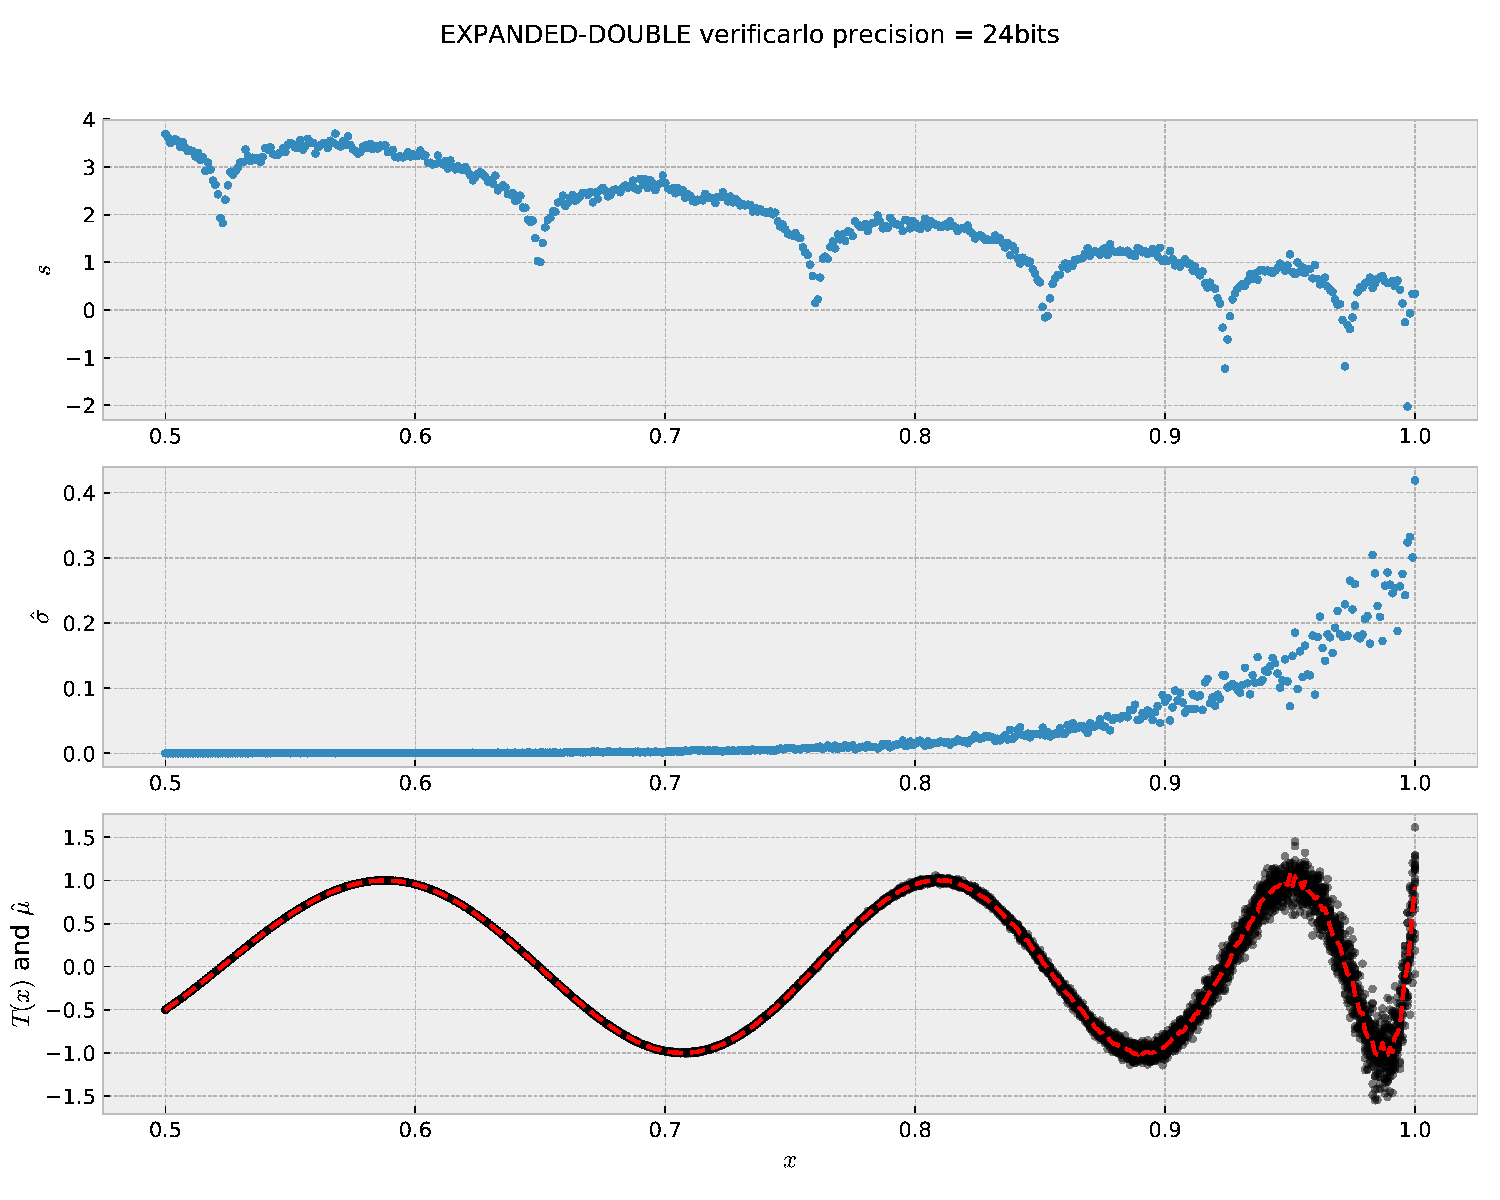
\includegraphics[width=.8\textwidth]{EXPANDED-DOUBLE-24.pdf}
  \caption{Evaluation of T(x) in its expanded form, compiled in double precision, with a virtual precision of 24}
  \label{fig:expanded:double:24}
\end{figure}
\begin{figure}[h]
\center 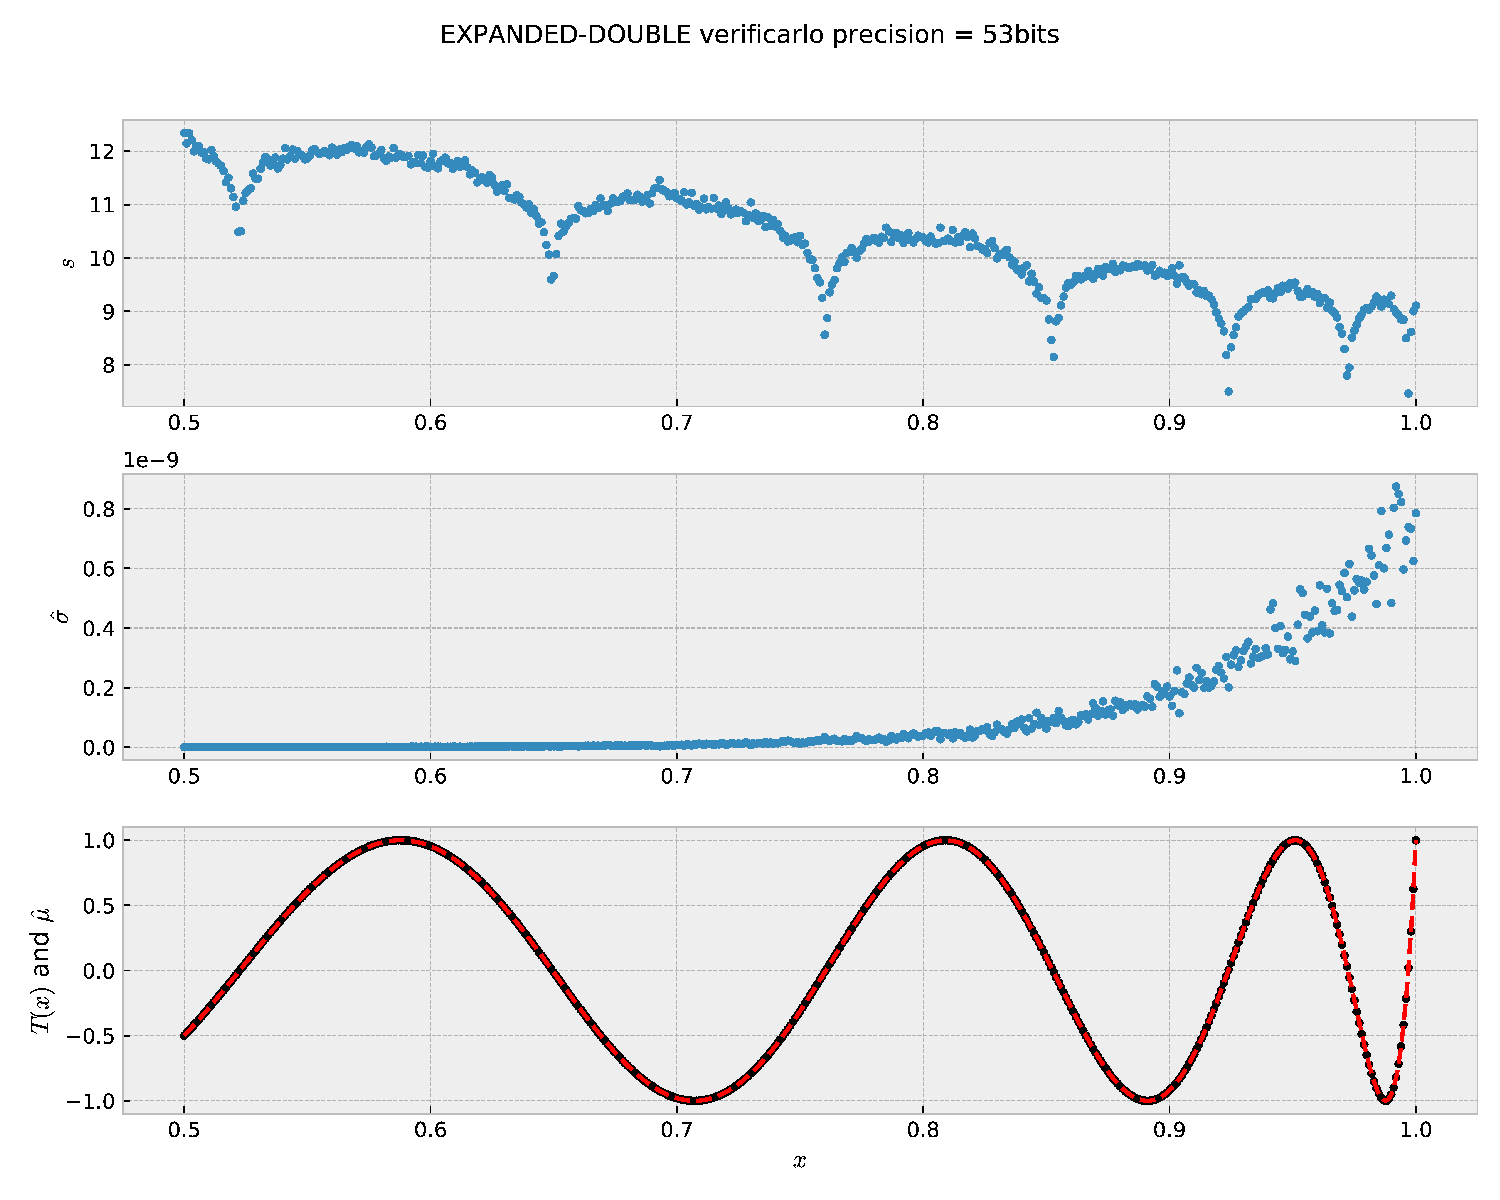
\includegraphics[width=.8\textwidth]{EXPANDED-DOUBLE-53.pdf}
  \caption{Evaluation of T(x) in its expanded form, compiled in double precision, with a virtual precision of 53}
  \label{fig:expanded:double:53}
\end{figure}

Close to 1, the polynomial evaluation is subject to {\it cancellations} which rapidly decrease the result precision. The double precision on the contrary seems satisfactory.

However using double precision is just moving the problem closer to 1 and it forces the programmer to use a larger and more costly data type.

Nevertheless if the user is already using double precision number, and if the precision is still not satisfactory, how to solve the issue? Or what if we need to use single precision?

\FloatBarrier

\subsection{Evaluation using Horner scheme}

It exists many other ways to evaluate polynomials, using associativity, commutativity and factorization. More often they are explored for sake of performance, but they also greatly influence the precision of the evaluation. One of them reputed to both performance with good numerical behavior is the Horner scheme which for our polynomial correspond to the following form:
% Horner reputed for good numerical behavior?

\[
	T(x) = (\dots((a_n\times x^2 + a_{n-1})\times x^2 + a_{n-2})\dots) \times x^2
    + a_0
\]

$$T(x) = (((((((((524288*x^2-2621440)*x^2+5570560)*x^2-6553600)*$$
$$x^2+4659200)*x^2-2050048)*x^2+549120)*x^2-84480)*$$
$$x^2+6600)*x^2-200)*x^2+1$$

\begin{question}
  \begin{enumerate}[(a)]
  \item Open the file {\tt tchebychev.c} and have a look to the function {\tt REAL horner(REAL x)}
\item While keeping previous execution parameters, execute the command {\tt ./run.sh HORNER DOUBLE 53}.  \newline The output of this command is given in figure~\ref{fig:horner:double:53}.
  \end{enumerate}
\end{question}

\begin{question}
 \item Modify the {\tt run.sh} script to evaluate the polynomial from $0.5$ to $1$ by $0.001$.
\item Execute the command {\tt ./run.sh HORNER DOUBLE 24}  \newline
The output of this command is given in figure~\ref{fig:horner:double:24}.

\end{question}

As shown in this experiment, the Horner scheme has a limited influence on the result precision ($\simeq$ 1 more bit). However, it minimizes the number of operations and allows to use the FMA ({\it Fused Multiply Add}). For a polynomial of degree $n$, it produces $n-1$ FMA. Moreover, when doing multiple independent evaluations it can be vectorized.


\begin{figure}[htb]
\center 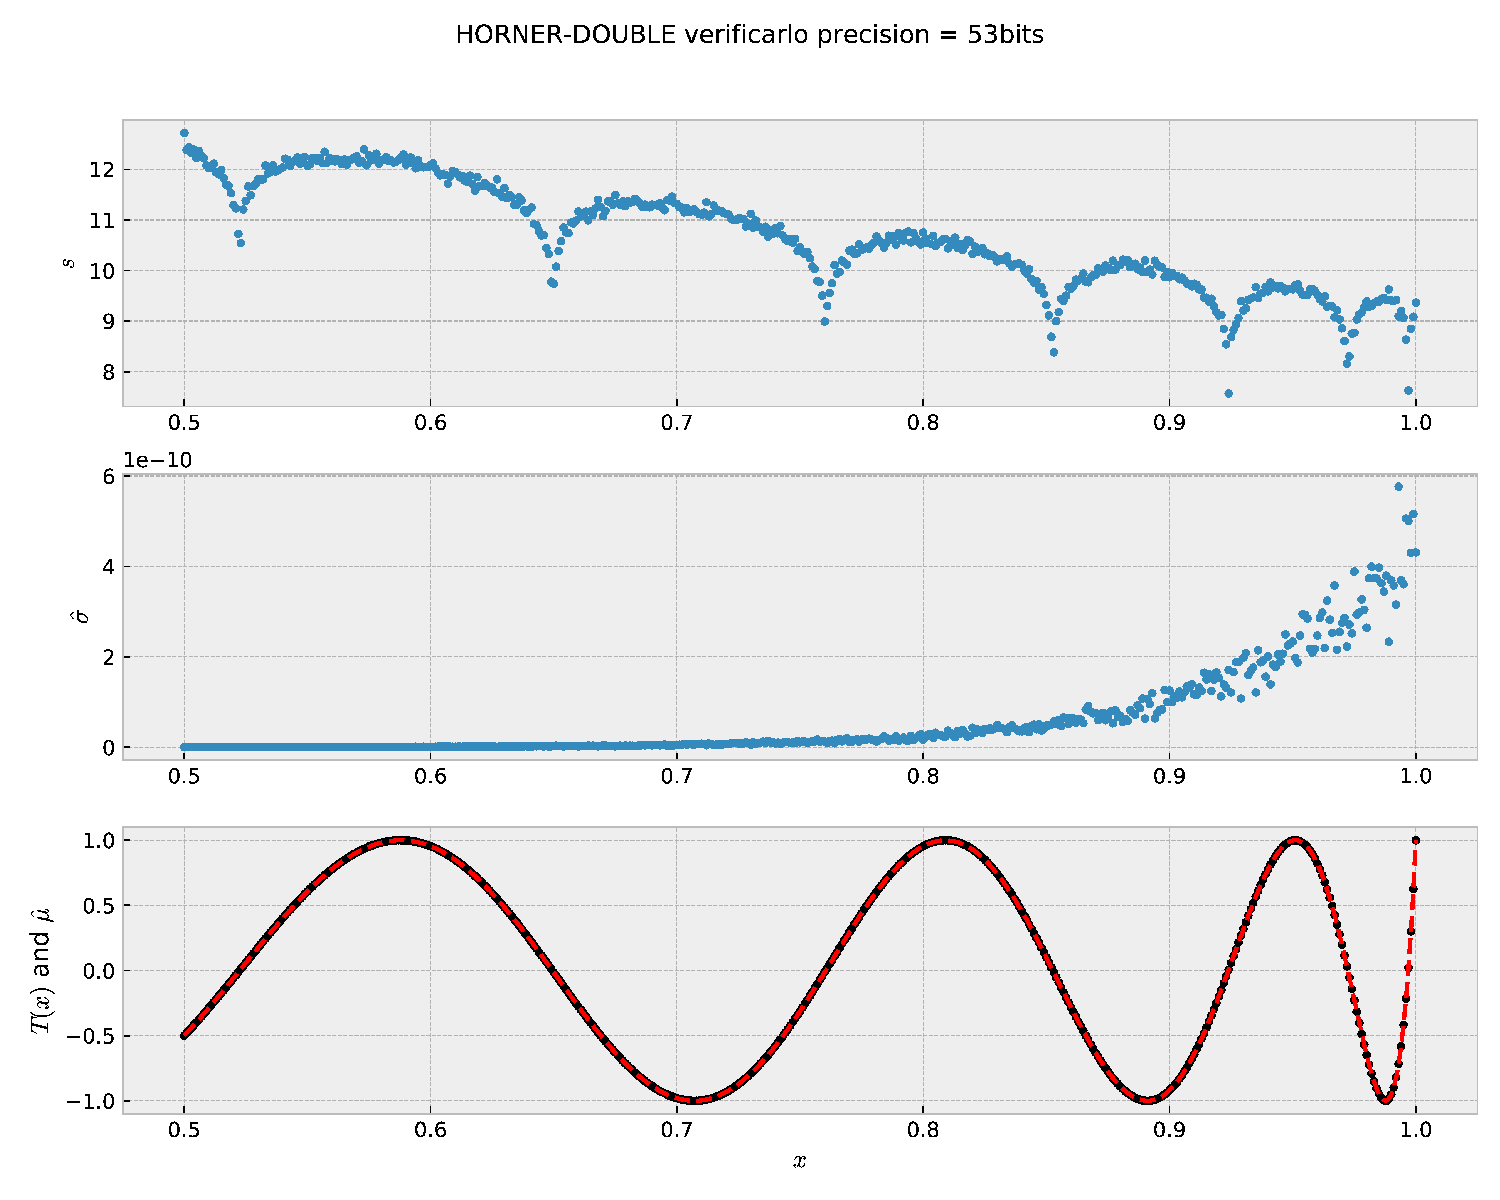
\includegraphics[width=.8\textwidth]{HORNER-DOUBLE-53.pdf}
  \caption{Evaluation of T(x) using Horner scheme, compiled in double precision, with a virtual precision of 53}
  \label{fig:horner:double:53}
\end{figure}
\begin{figure}[htb]
\center 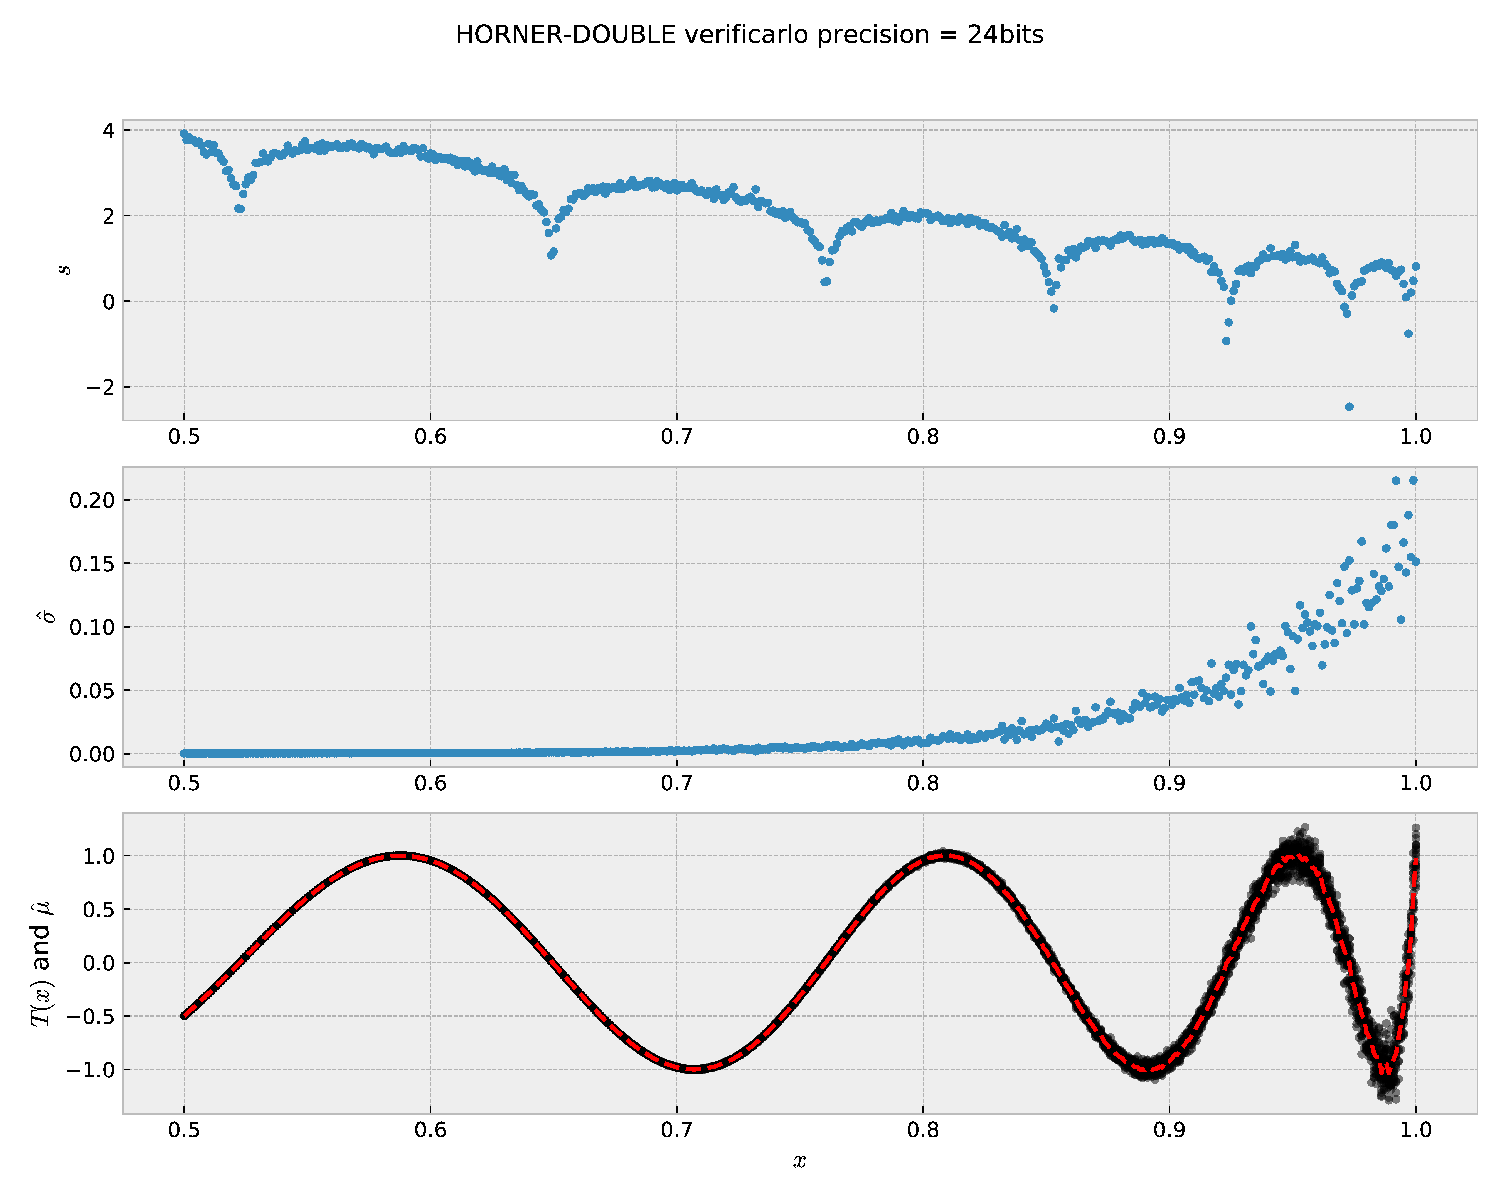
\includegraphics[width=.8\textwidth]{HORNER-DOUBLE-24.pdf}
  \caption{Evaluation of T(x) using Horner scheme, compiled in double precision, with a virtual precision of 24}
  \label{fig:horner:double:24}
\end{figure}


\FloatBarrier

\subsection{Factored form}

We will now evaluate the evaluation precision of the following factored rewriting:
\[
	T(x) = 1 + 8x^2\,(x-1)\,(x+1)\,(4x^2 + 2x - 1)^2\, (4x^2 - 2x - 1)^2\,(16x^4 - 20x^2 + 5)^2
\]

\begin{eqnarray*}
T(x) &=& 8.0*x^2*(x - 1.0)*(x + 1.0) \\
 & & * (4.0*x^2 + 2.0*x - 1.0)*(4.0*x^2 + 2.0*x - 1.0) \\
 & & * (4.0*x^2 - 2.0*x - 1.0)*(4.0*x^2 - 2.0*x - 1.0)* \\
 & & * (16.0*x^4 - 20.0*x^2 + 5.0)*(16.0*x^4 - 20.0*x^2 + 5.0) + 1 \\
\end{eqnarray*}

\begin{question}
  \begin{enumerate}[(a)]
  \item Open the file {\tt tchebychev.c} and have a look to the function {\tt REAL factored (REAL x)}
\item Execute the command {\tt ./run.sh FACTORED DOUBLE 24} \newline
The output of this command is given in figure~\ref{fig:factored:double:24}.
\item Compare these results to those obtained with EXPANDED and HORNER versions.
  \end{enumerate}
\end{question}

\begin{figure}[h]
\center 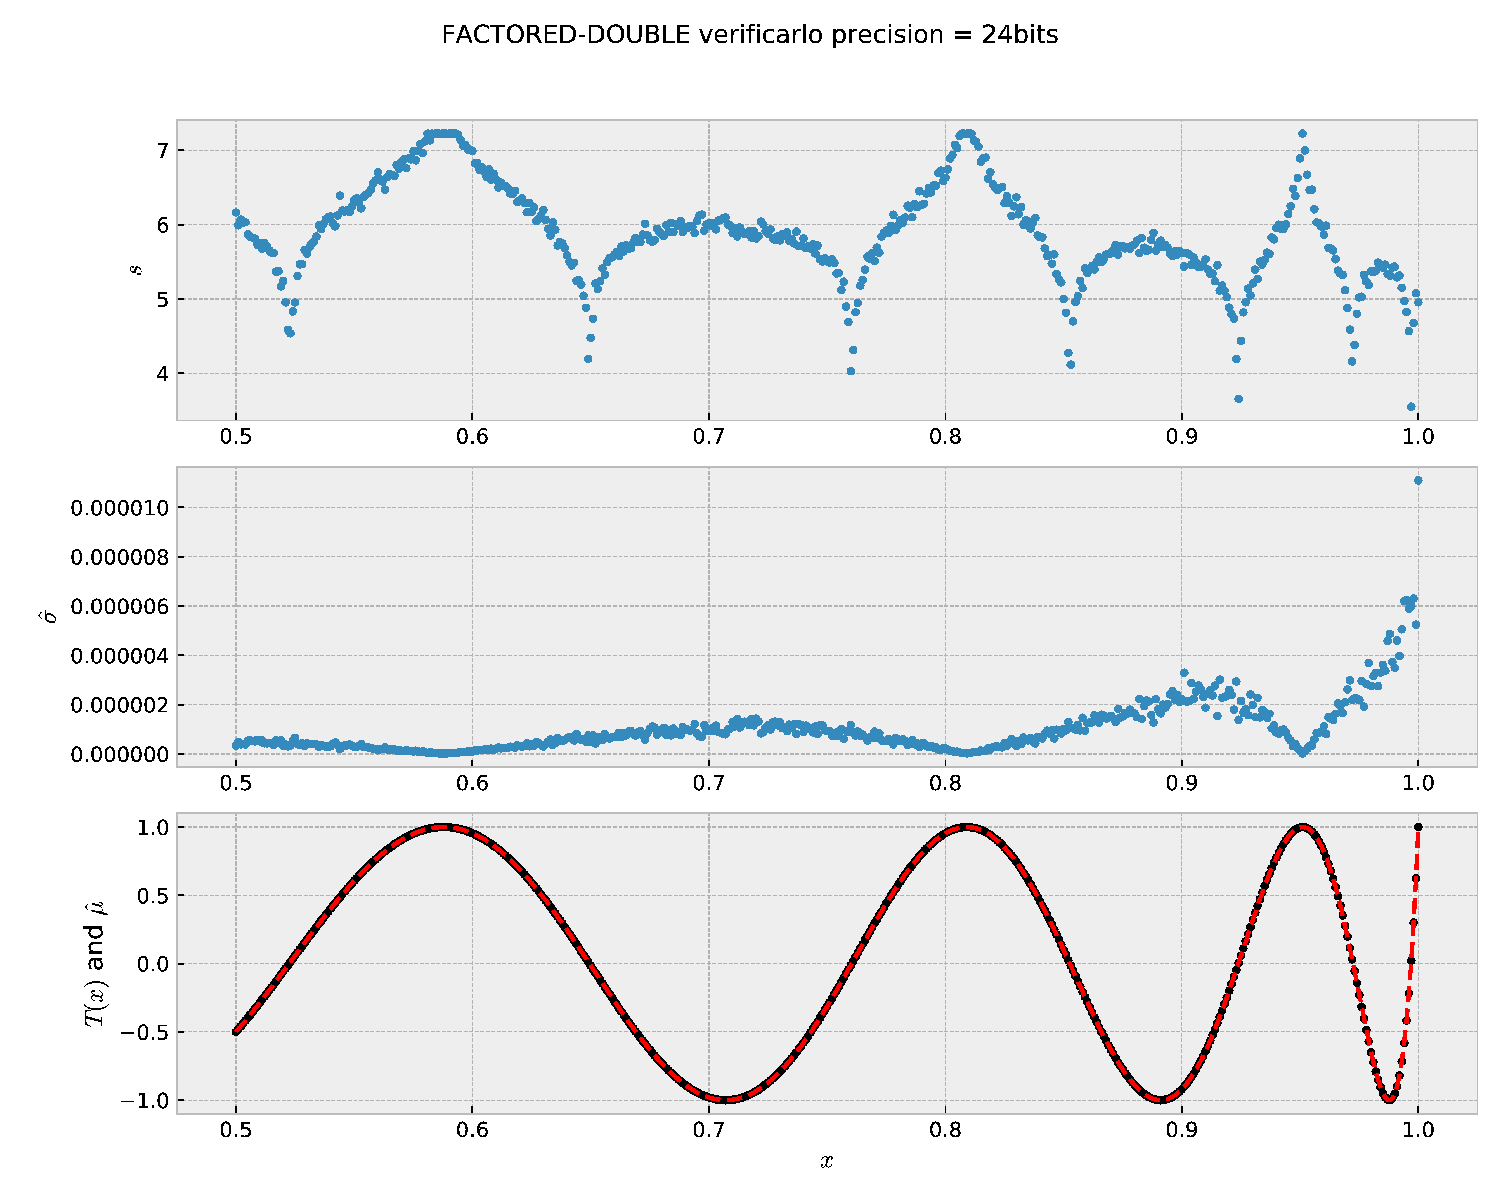
\includegraphics[width=.8\textwidth]{FACTORED-DOUBLE-24.pdf}
  \caption{Evaluation of T(x) in its factored form, compiled in double precision, with a virtual precision of 24}
  \label{fig:factored:double:24}
\end{figure}

\begin{question}
  Explain what happens when $T(x)=1$ for $x\simeq 0.6$,
  $x\simeq 0.8$ et $x\simeq 0.95$.\\~\\
  $\rightarrow$ It is an example where the error is absorbed and the precision and accuracy  of the results are improved.
\end{question}


\begin{question}
  \begin{enumerate}[(a)]
    \item Modify the {\tt run.sh} script to evaluate the  polynomial between $0.99$ and $1$ by $0.00001$ step.
  \item Run the scripts to execute and visualize the results for
    FACTORED, EXPANDED and HORNER with a virtual precision of 53. The results are respectively presented in figure~\ref{fig:factored:double:53:zoom},\ref{fig:expanded:double:53:zoom}
    and~\ref{fig:horner:double:53:zoom}.

\item Reproduce the result with a virtual precision of 24. The results are respectively presented in figure~\ref{fig:factored:double:24:zoom},\ref{fig:expanded:double:24:zoom}
    and~\ref{fig:horner:double:24:zoom}

\end{enumerate}
\end{question}

\begin{figure}[h]
  \center 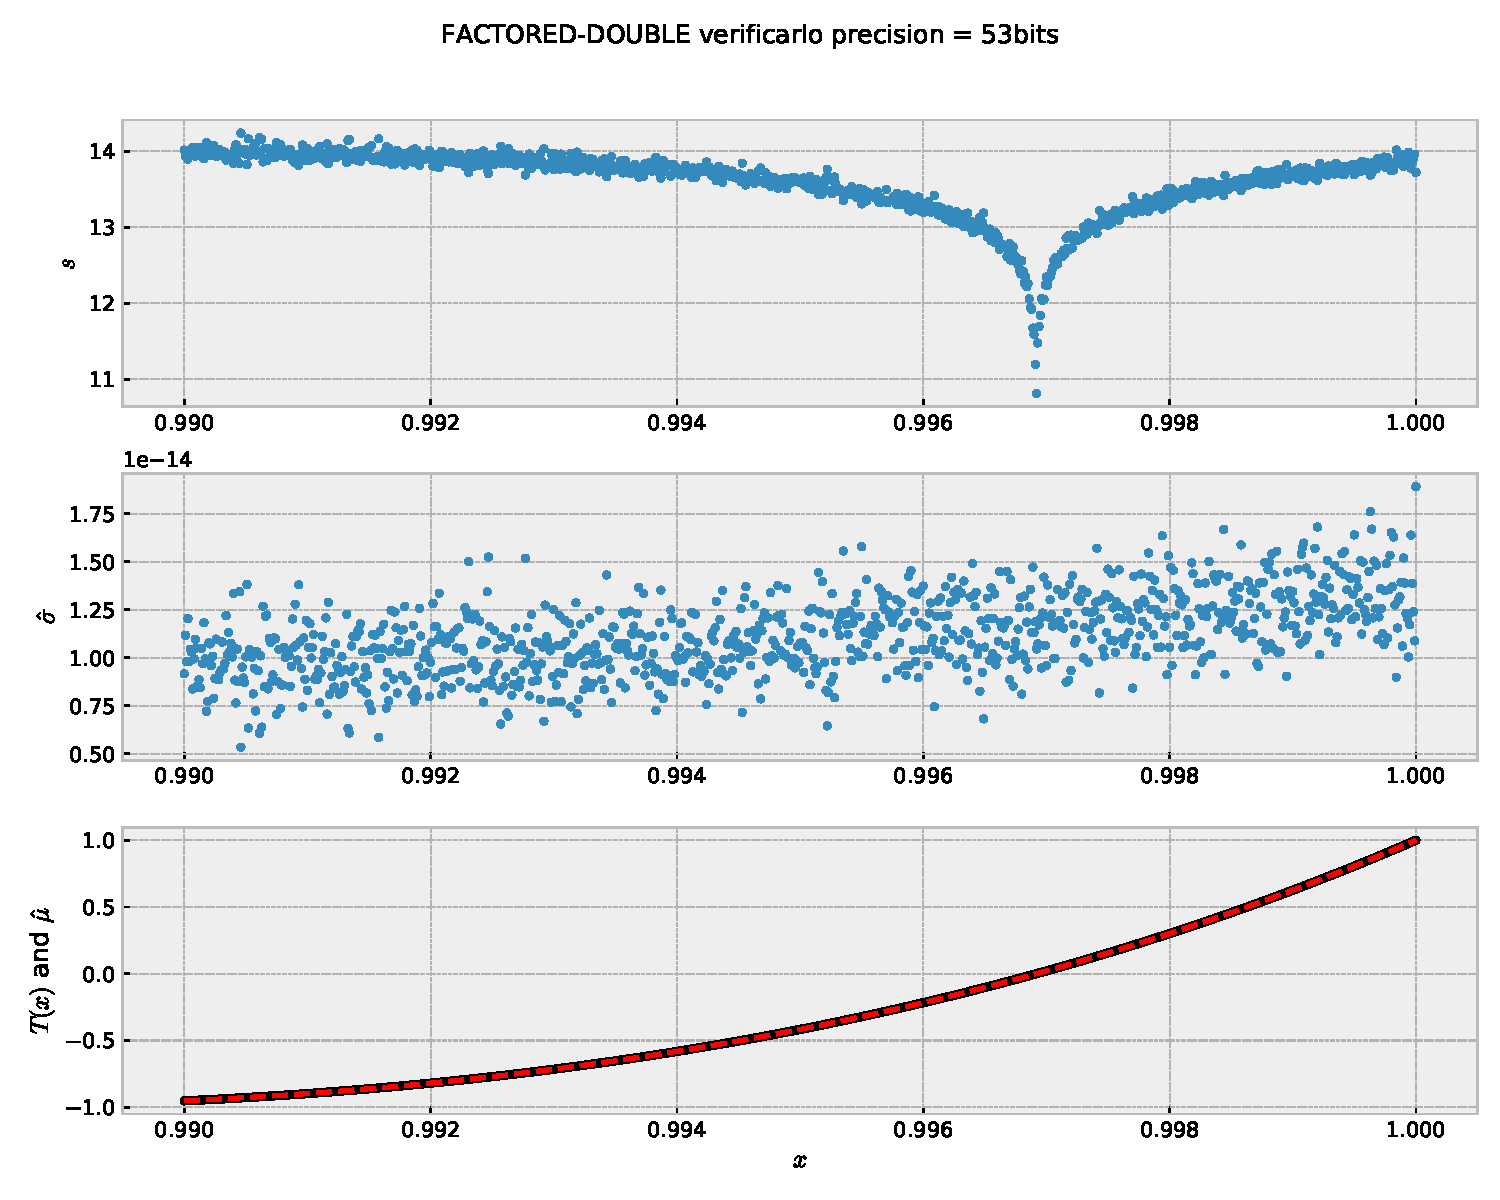
\includegraphics[width=.8\textwidth]{FACTORED-DOUBLE-53-zoom.pdf}
  \caption{Evaluation of T(x) in its factored form, compiled in double
    precision, with a virtual precision of 53}
  \label{fig:factored:double:53:zoom}
\end{figure}

\begin{figure}[h]
  \center 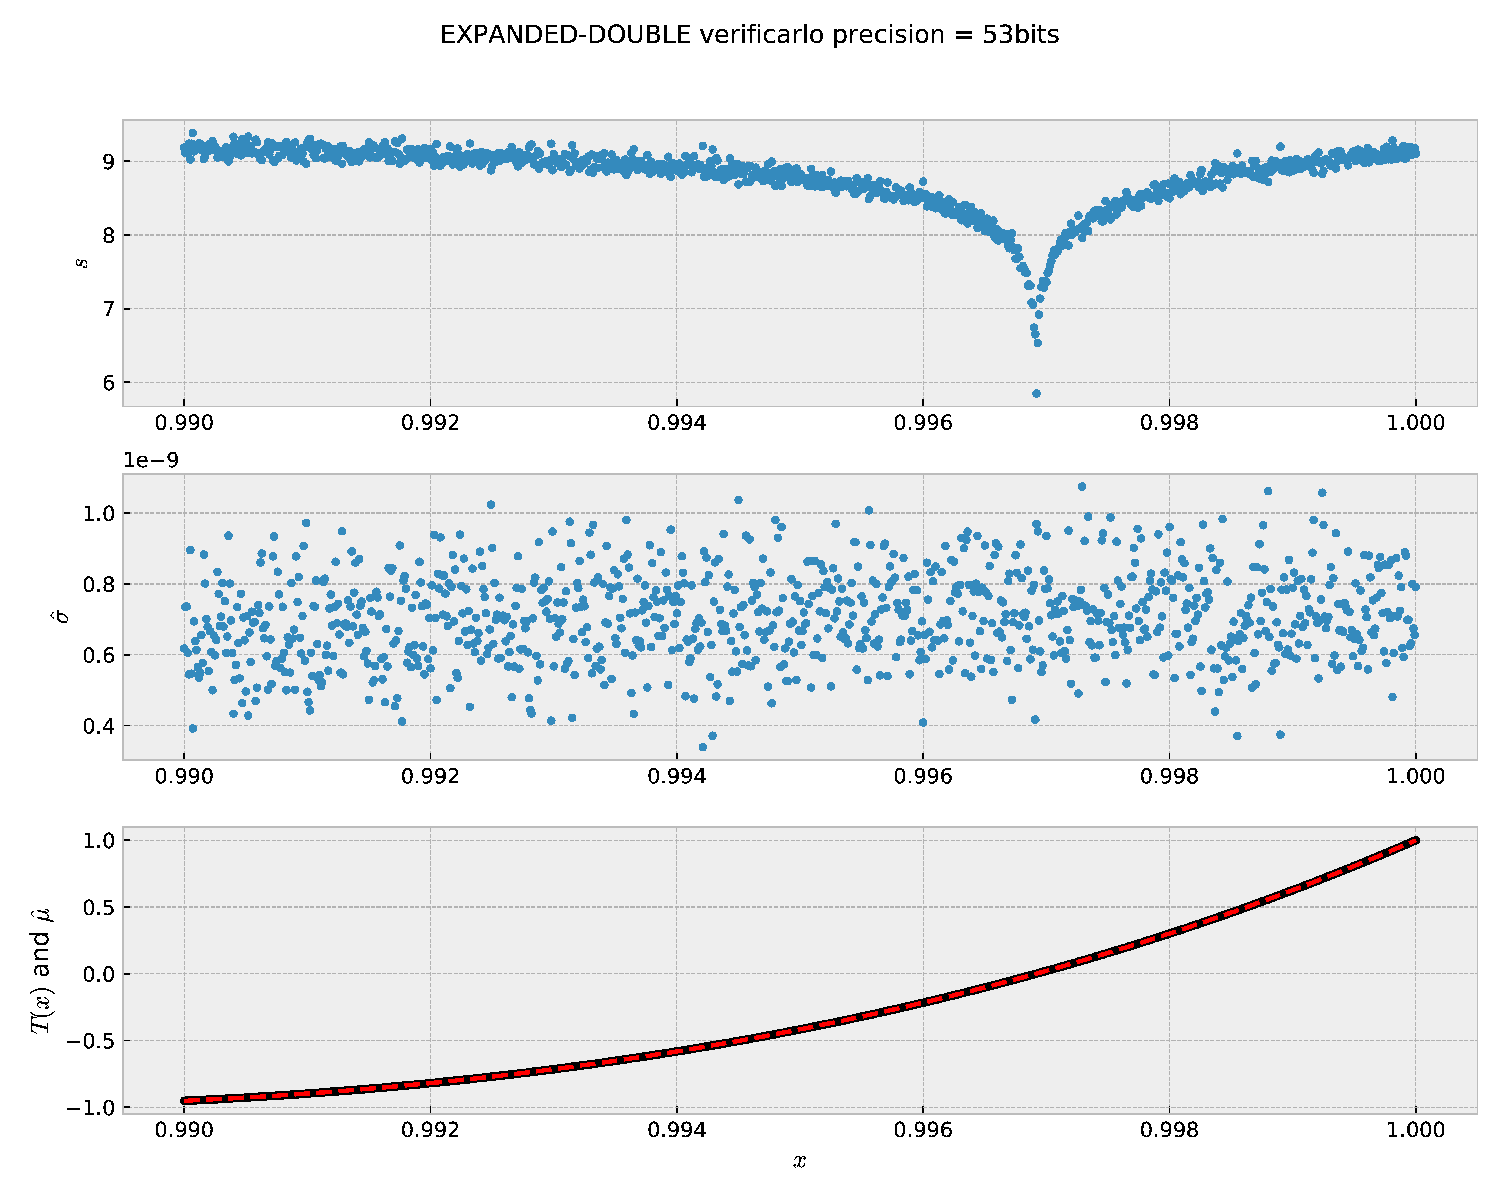
\includegraphics[width=.8\textwidth]{EXPANDED-DOUBLE-53-zoom.pdf}
  \caption{Evaluation of T(x) in its expanded form, compiled in double
    precision, with a virtual precision of 53}
  \label{fig:expanded:double:53:zoom}
\end{figure}

\begin{figure}[h]
  \center 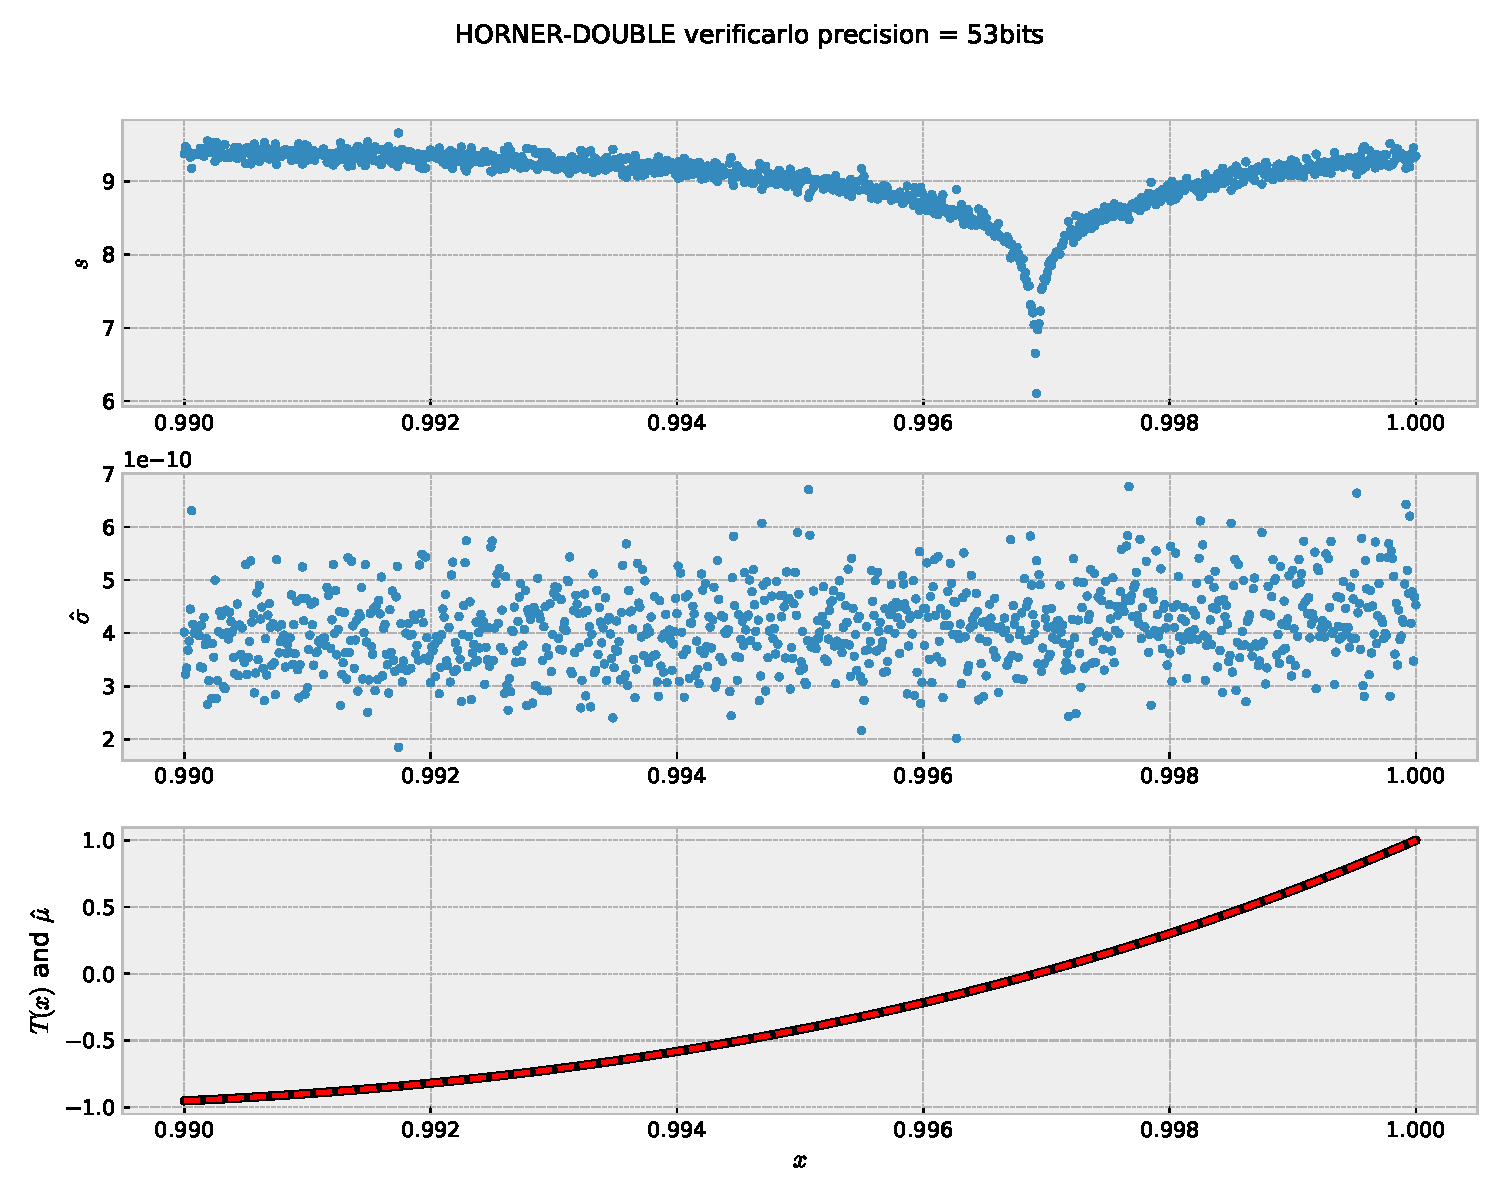
\includegraphics[width=.8\textwidth]{HORNER-DOUBLE-53-zoom.pdf}
  \caption{Evaluation of T(x) using Horner scheme, compiled in double precision,
    with a virtual precision of 53}
  \label{fig:horner:double:53:zoom}
\end{figure}

\begin{figure}[h]
  \center 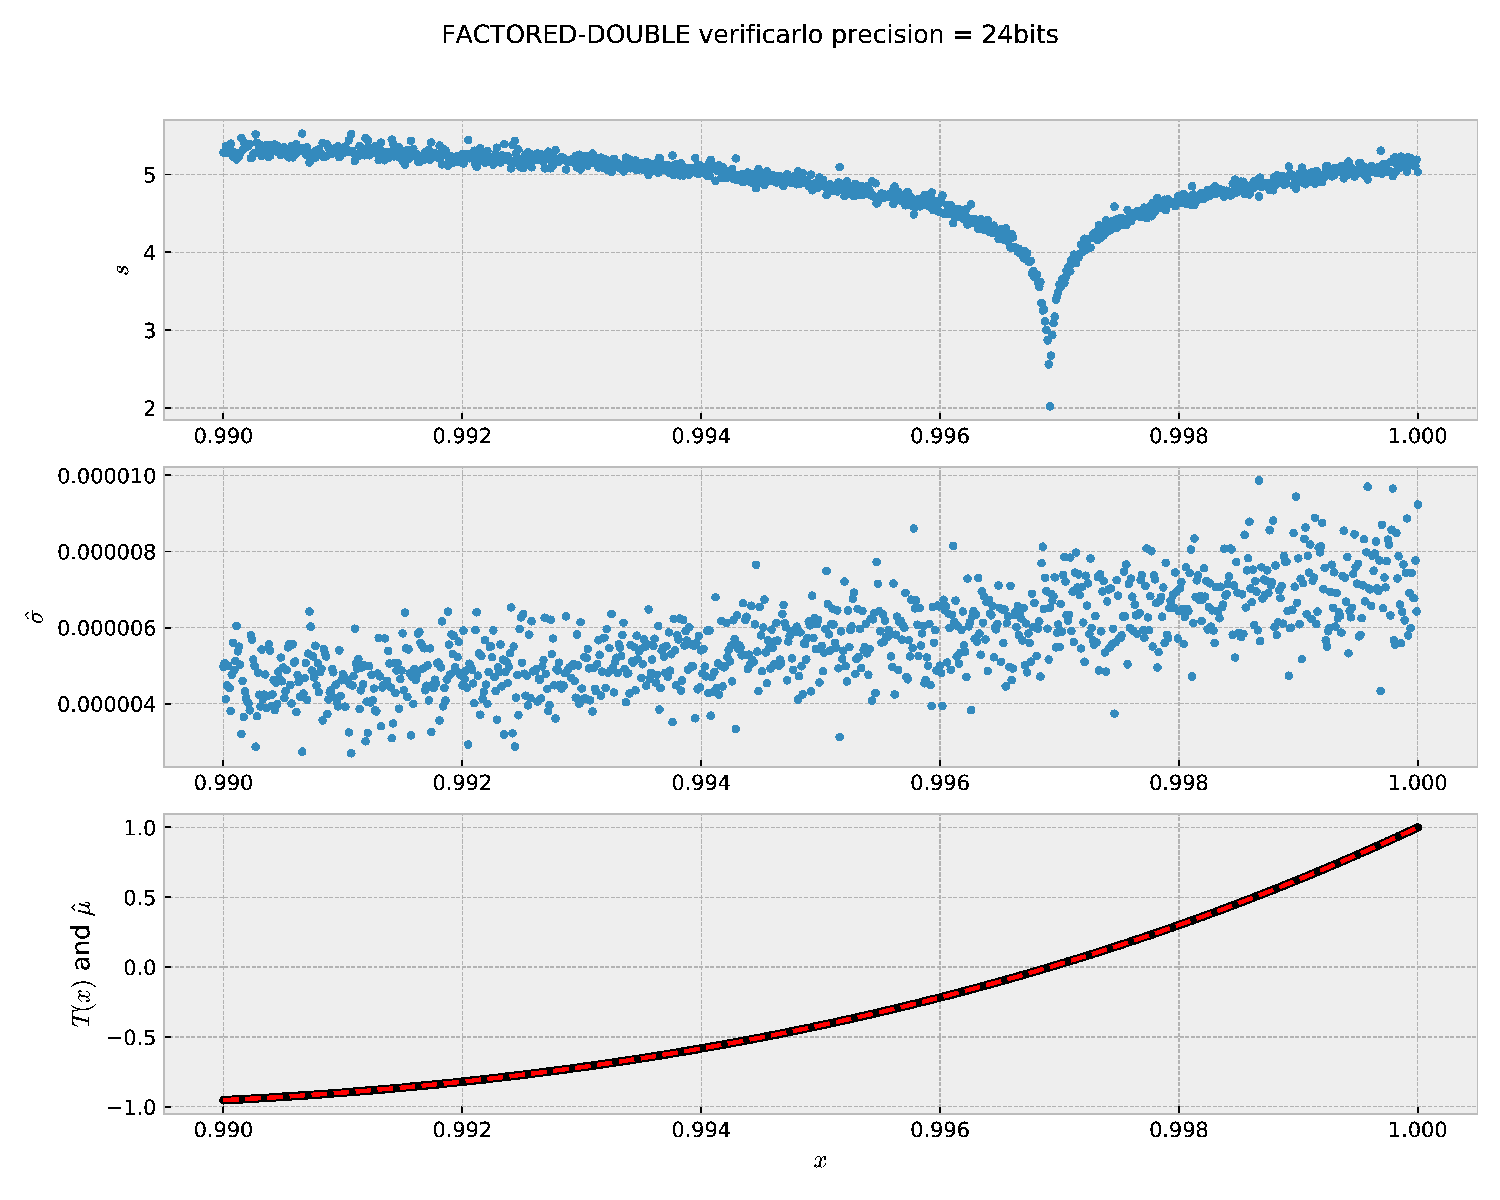
\includegraphics[width=.8\textwidth]{FACTORED-DOUBLE-24-zoom.pdf}
  \caption{Evaluation of T(x) in its factored form, compiled in double
    precision, with a virtual precision of 24}
  \label{fig:factored:double:24:zoom}
\end{figure}

\begin{figure}[h]
  \center 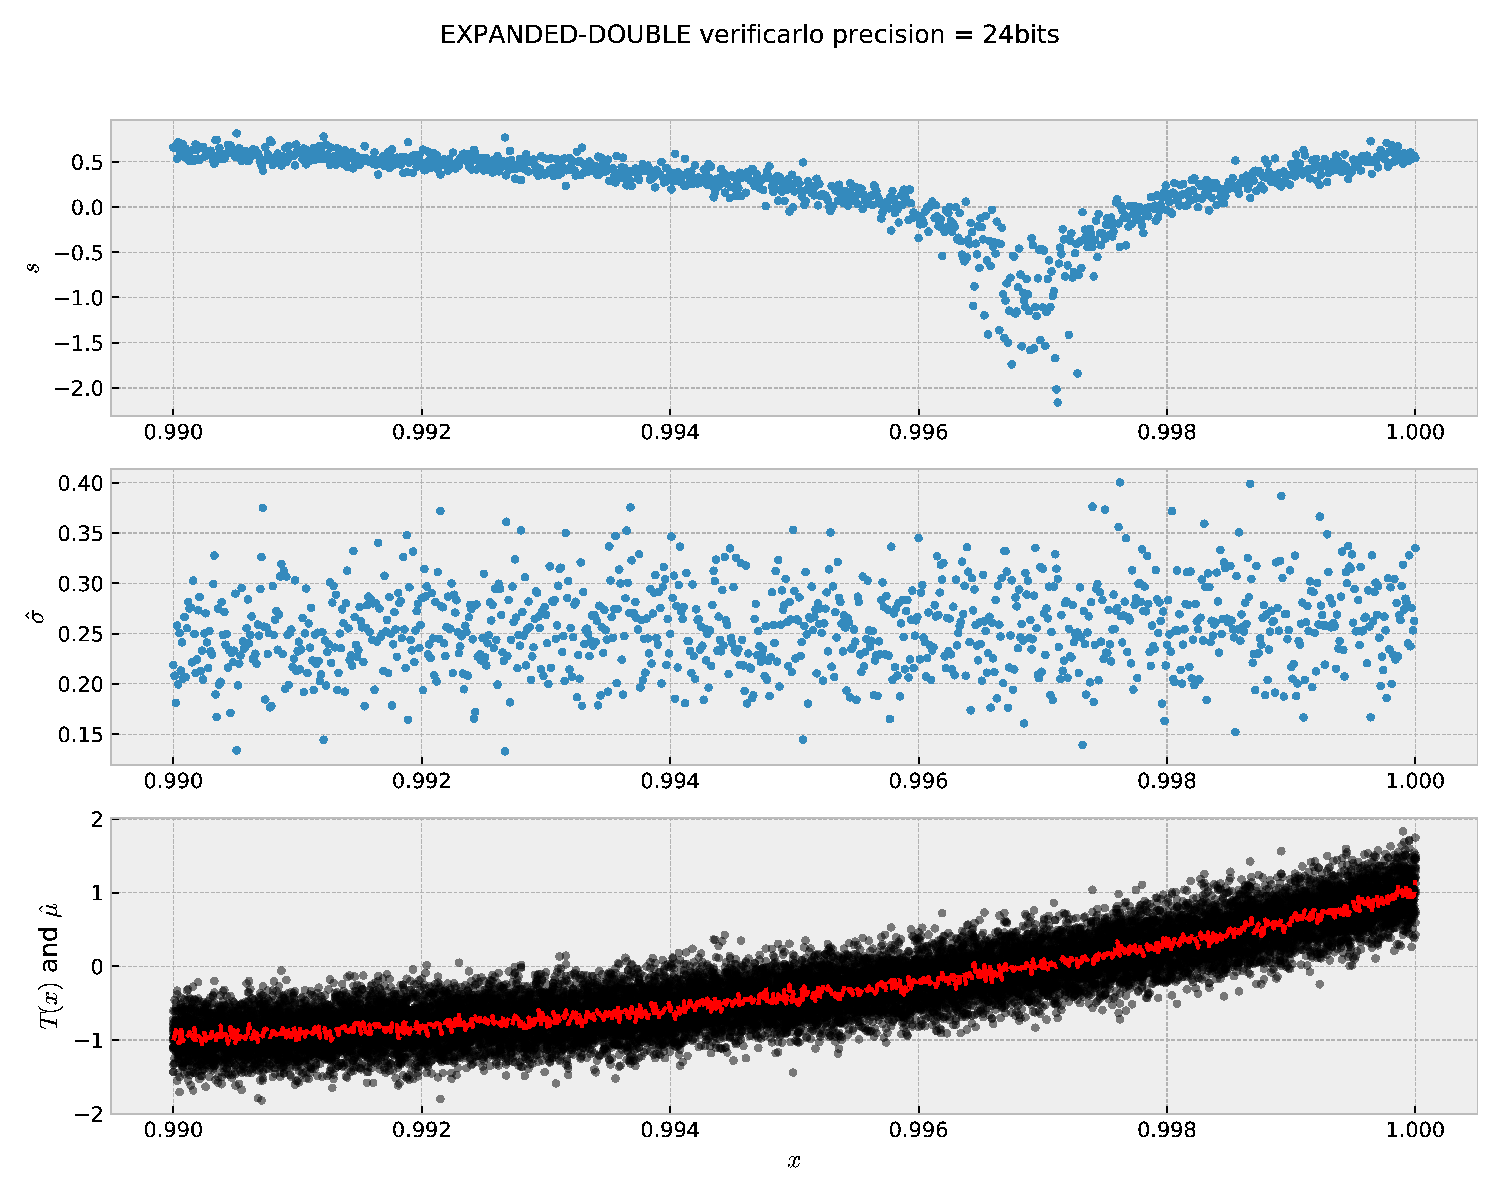
\includegraphics[width=.8\textwidth]{EXPANDED-DOUBLE-24-zoom.pdf}
  \caption{Evaluation of T(x) in its expanded form, compiled in double
    precision, with a virtual precision of 24}
  \label{fig:expanded:double:24:zoom}
\end{figure}

\begin{figure}[h]
  \center 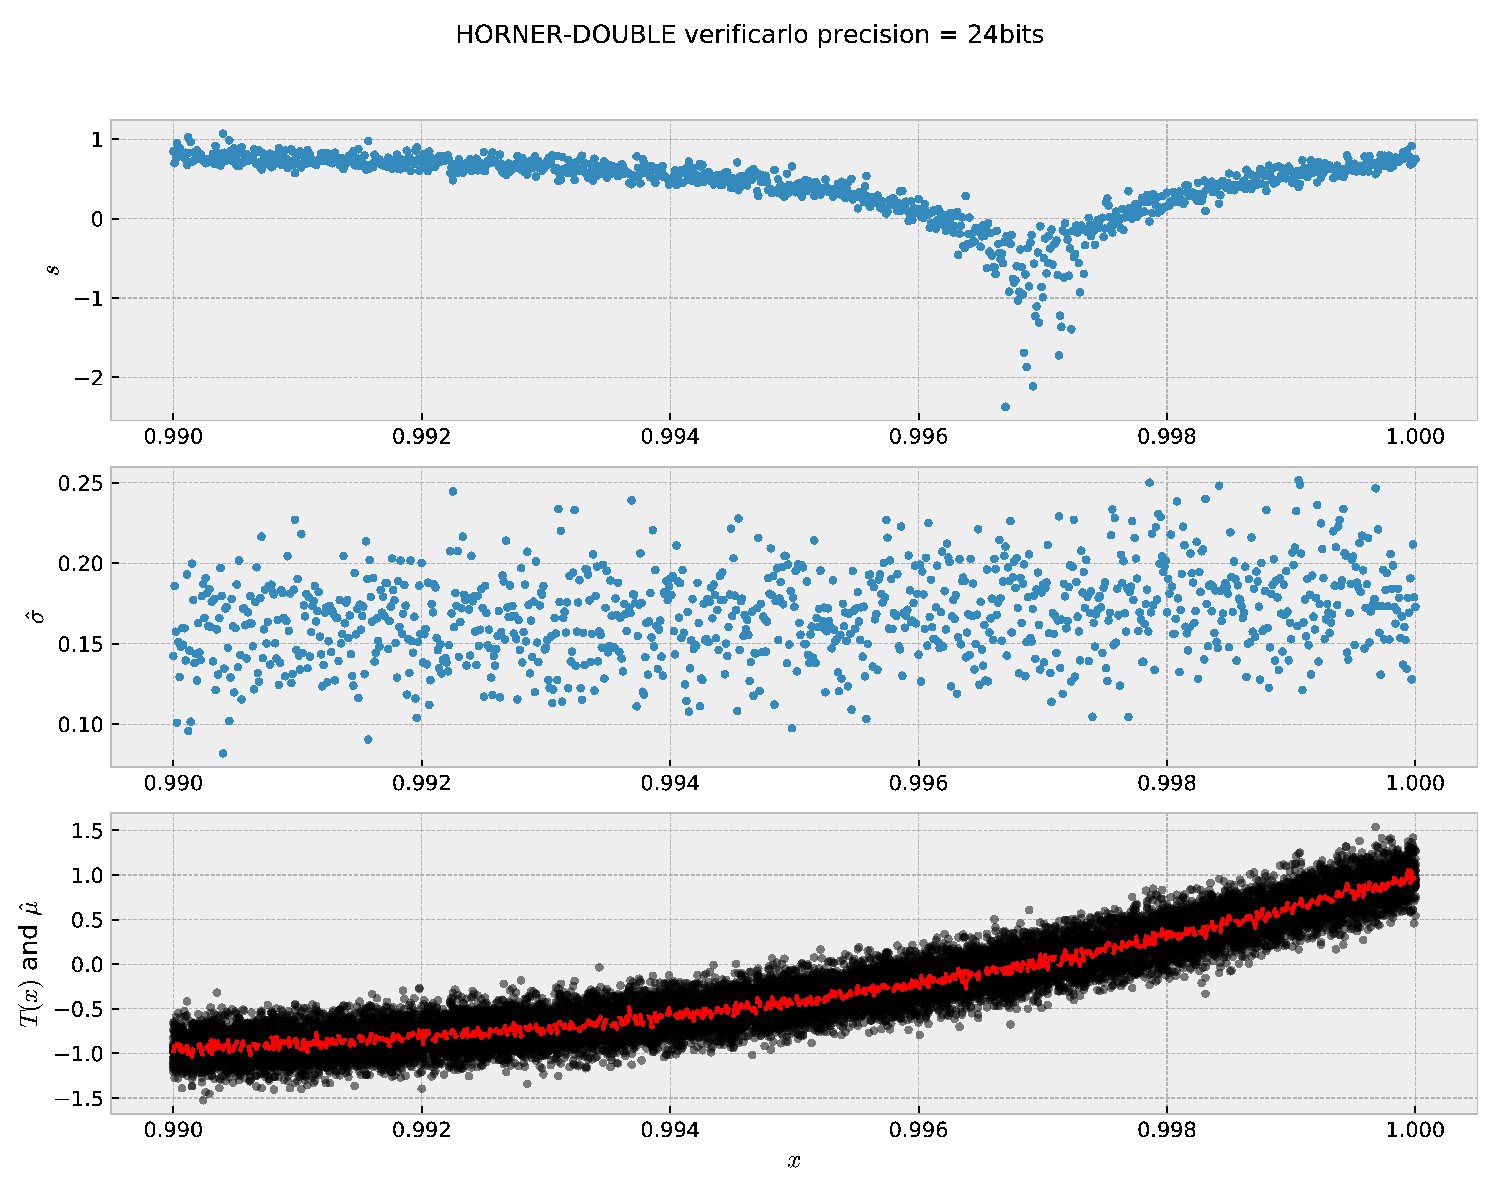
\includegraphics[width=.8\textwidth]{HORNER-DOUBLE-24-zoom.pdf}
  \caption{Evaluation of T(x) using Horner scheme, compiled in double precision,
    with a virtual precision of 24}
    \label{fig:horner:double:24:zoom}
\end{figure}

\subsection{Conclusion}


From a general stand point, for every arithmetic expression in a program, it exists many valid rewriting. They are not all equivalent in terms of performance, precision, and accuracy!

\begin{question}
What is the best approach?
\end{question}

\FloatBarrier

